
To better understand how coordination facts are used, we next present some programs that
take advantage of them.

\subsection{Single Source Shortest Path}

The Single Source Shortest Path (SSSP) program was already presented in
Section~\ref{sec:language}. We are going to update the code in
Fig.~\ref{code:shortest_path_program} so that nodes with the shortest distances
are selected to run before others nodes. The coordinated version of the same
algorithm is presented in Fig.~\ref{code:shortest_path_program_coord} and it
uses one coordination fact, namely \texttt{set-priority} (line 15). Note that we
also use a global program directive to order priorities in ascending order (line
5).

When using a single thread, the algorithm behaves like
Dijkstra's shortest path algorithm~\cite{Dijkstra}. However, when using multiple
threads, each thread will pick the smallest distance from their subset of nodes.
While this is not optimal since threads do not share a global view of priorities,
many rule derivations are going to be avoided.

\begin{figure}[h!]
\scriptsize\begin{Verbatim}[numbers=left,commandchars=&\[\]]
type route edge(node, node, int).
type linear shortest(node, int, list int).
type linear relax(node, int, list int).

&underline[priority @order asc].

shortest(A, +00, \[\]).
relax(@1, 0, [@1]).

relax(A, D1, P1), shortest(A, D2, P2),
D1 < D2
   -o shortest(A, D1, P1),
      {B, W | !edge(A, B, W) |
         relax(B, D1 + W, P1 ++ \[B\]),
         &underline[set-priority(B, float(D1 + W))]}.

relax(A, D1, P1), shortest(A, D2, P2),
D1 >= D2
   -o path(A, D2, P2).
\end{Verbatim}
  \caption{Shortest Path Program.}
  \label{code:shortest_path_program_coord}
\end{figure}
\normalsize

\begin{figure}[h!]
   \begin{center}
      \subfloat[]{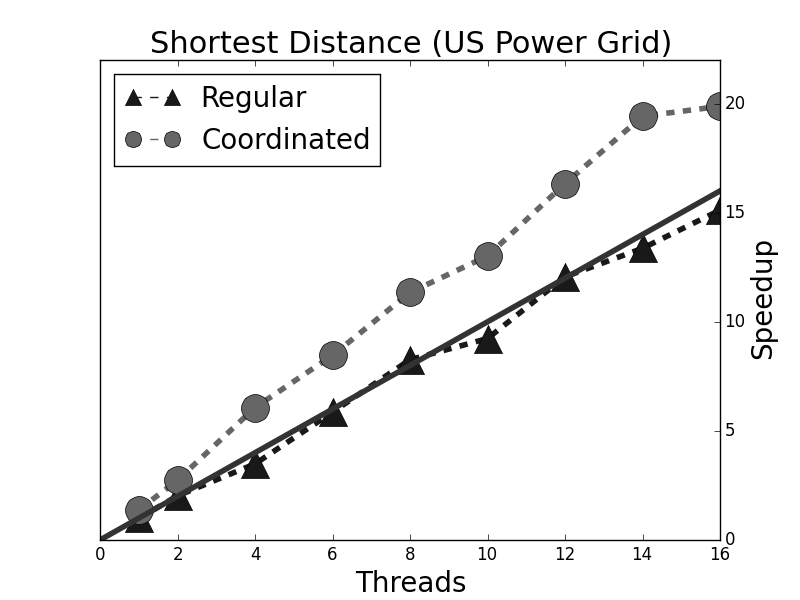
\includegraphics[width=4cm]{results/shortest-uspowergrid.png}}
      \subfloat[]{ \scriptsize\begin{tabular}{ | c | c | c | }
         \hline                       
         \textbf{\# T} & \textbf{R} & \textbf{C} \\ \hline \hline
         1 & 333K & 206K \\
         2 & 300K & 210K \\
         4 & 316K & 208K \\
         8 & 328K & 211K \\
         16 & 343K & 212K \\
         \hline  
         \end{tabular}
         \normalsize
      }
   \end{center}
   \caption{Single Source Shortest Path program code.}
   \label{results:sssp_uspowergrid}
\end{figure}

\subsection{Graph Search}


\subsection{MiniMax}

\begin{figure}[h!]
   \begin{center}
      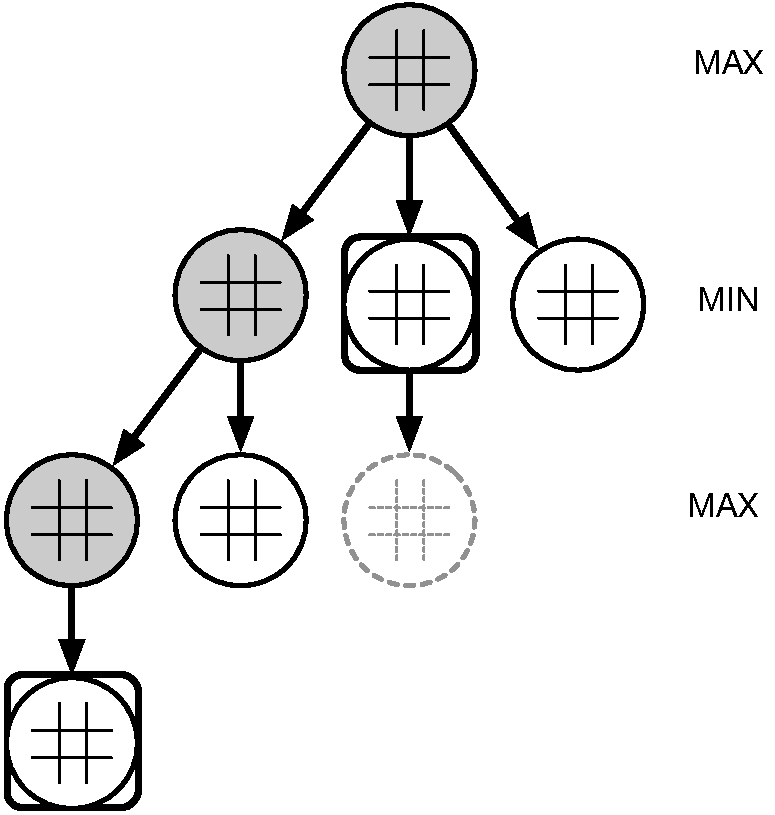
\includegraphics[width=5cm]{figures/minimax_tree}
   \end{center}
   \caption{Single Source Shortest Path program code.}
   \label{minimax}
\end{figure}


\subsection{Heat Transfer}

\subsection{Splash BP}

Randomized and approximation
algorithms can obtain significant benefits from coordination directives because although the final
program results will not be exact, they follow important statistical properties and can be computed faster.
Examples of such programs are PageRank~\cite{Lubachevsky:1986:CAA:4904.4801} and
Loopy Belief Propagation~\cite{Gonzalez+al:aistats09paraml}.

Loopy Belief Propagation~\cite{Murphy99loopybelief} (LBP) is an approximate inference algorithm
used in graphical models with cycles. In its essence, LBP is a sum-product message passing algorithm
where nodes exchange messages with their immediate neighbors and apply some computations to the messages
received.

LBP is an algorithm that maps very well to the graph based model of LM. In its original form, we need to compute
the belief of all nodes for several iterations and also synchronize after each iteration.
However, it is still possible to apply
some optimizations in order to take advantage of the fact that LBP will converge even when using
an asynchronous approach. So, instead of computing the belief iteratively,
we first keep track of all messages sent/received (and overwrite them when we receive a new one)
and recompute the belief when we want, instead of synchronizing between nodes.
This way, we can prioritize the computation of beliefs when
a node's belief value changes significantly. When that happens, we set the priority of its
neighbors so that they can recompute their beliefs.

The asynchronous approach proves to be a nice improvement over the synchronous version. Still, it
is possible to do even better. Gonzalez et al~\cite{Gonzalez+al:aistats09paraml} developed an optimal
algorithm to compute this algorithm by first building a tree and then updating the beliefs of each node twice, first from the leaves to the root and then from the root to the leaves. The root of this tree
is the node with the highest priority (based on belief) while the other nodes in the tree
must have a non-zero priority. Note that the priorities are updated whenever a neighbor updates
their belief. These splash trees are built iteratively until we reach convergence.

\begin{figure}[h!]
   \begin{center}
      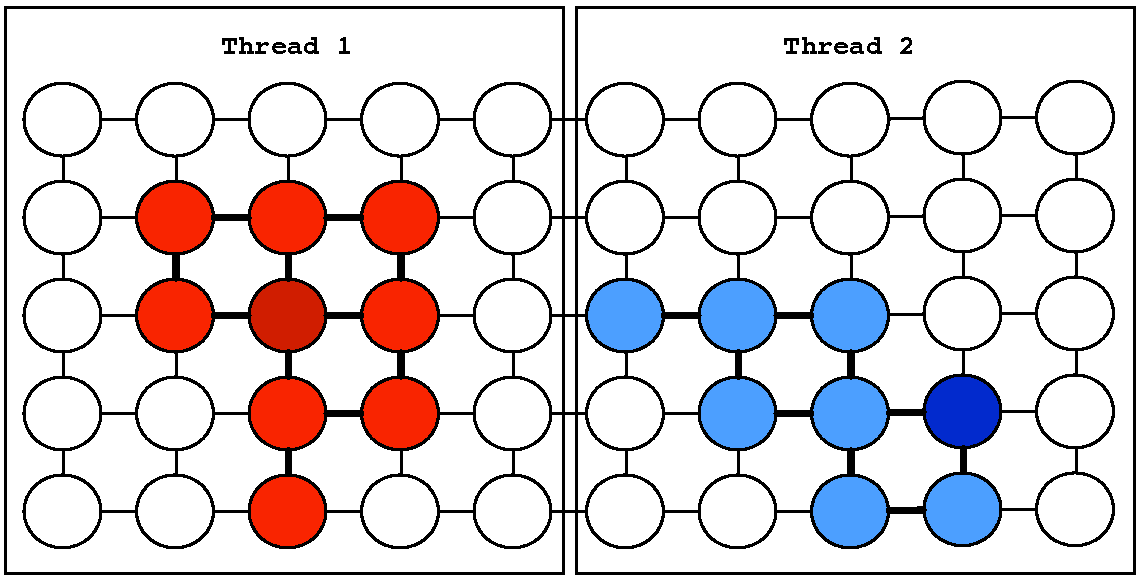
\includegraphics[width=6.5cm]{figures/splash_bp}
   \end{center}
   \caption{Single Source Shortest Path program code.}
   \label{splash_bp}
\end{figure}


The code in Fig.~\ref{code:sbp} presents the coordination code of the Belief Propagation problem.
Please note that we just appended the code in Fig.~\ref{code:sbp} to a working but
unoptimized version of the algorithm.
In the coordination code we have three sections:
\begin{description}
   \item[Tree building]: Each node has a \texttt{waiting} fact that is used to start the tree building process. When the highest priority is picked we create a token that will navigate through the tree. Note that in the rule located in lines 11-18 we check if the priority of the new node to add to the tree is positive and that both nodes are in the same thread. We want the tree to be kept in the same thread.
   \item[First phase]: In the third rule (lines 8-9), when we reach a certain number of nodes in the tree, we generate \texttt{first-phase} in order to update the beliefs of all nodes in tree starting from the leaves and ending at the root. As we update the nodes, we generate \texttt{update} to update the belief values (line 29).
   \item[Second phase]: In the second phase we go from the root to the leaves and update the beliefs a second time (line 39).
\end{description}

When we have several threads, every thread will generate their own trees by taking into account the highest priority node in their own queues.

\begin{figure}[h!]
\scriptsize\begin{Verbatim}[numbers=left,commandchars=*\{\}]
set-static(A). // all nodes are static.

// TREE BUILDING
// continue tree
waiting(A), token(A, All, Next) -o token(A, All, Next).
// start tree
waiting(A), *underline{@priority(A, A, P)}, P > 0.0
   -o token(A, [A], [A]).
// end tree building
token(A, All, Next), length(All) > maxnodes
   -o first-phase(A, All, reverse(All)).
// expand tree
token(A, All, [A | Next])
   -o [collect => L | Side | !edge(A, L, Side),
         0 = count(All, L),
         0 = count(Next, L),
         *underline{priority(A, L, P)}, P > 0.0,
         *underline{cpu-id(A, L, Id1)},
         *underline{cpu-id(A, A, Id2)}, Id1 = Id2 |
         send-token(A, All, Next ++ L)].

send-token(A, All, [])
   -o first-phase(A, All, reverse(All)).
send-token(A, All, [B | Next])
   -o *underline{schedule-next(B)},
      token(B, All ++ [B], [B | Next]).

// FIRST PHASE
first-phase(A, [A], [A]) -o second-phase(A, [], A).
first-phase(A, [A, B | Next], [A])
   -o update(A), *underline{schedule-next(B)},
      second-phase(B, [B | Next], A).
first-phase(A, All, [A, B | Next])
   -o update(A), *underline{schedule-next(B)},
      first-phase(B, All, [B | Next]).

// SECOND PHASE
second-phase(A, [], _)
   -o *underline{set-priority(A, 0.0)}, waiting(A), update(A).
second-phase(A, [A], Back)
   -o update(A), waiting(Back),
      waiting(A), *underline{set-priority(A, 0.0)}.
second-phase(A, [A, B | Next], Back)
   -o update(A), waiting(Back), *underline{schedule-next(B)},
      second-phase(B, [B | Next], A).
\end{Verbatim}
  \caption{Coordination code for the Splash Belief Propagation program.}
  \label{code:sbp}
\end{figure}
\normalsize
